%% LyX 2.1.3 created this file.  For more info, see http://www.lyx.org/.
%% Do not edit unless you really know what you are doing.
\documentclass[11pt,english]{article}
\renewcommand{\rmdefault}{cmr}
\renewcommand{\sfdefault}{cmss}
\renewcommand{\ttdefault}{cmtt}
\usepackage[T1]{fontenc}
\usepackage[latin9]{inputenc}
\usepackage{geometry}
\geometry{verbose,tmargin=2.5cm,bmargin=2.5cm,lmargin=2.5cm,rmargin=2.5cm}
\setlength{\parskip}{\bigskipamount}
\setlength{\parindent}{0pt}
\usepackage{babel}
\usepackage{amsthm}
\usepackage{amsmath}
\usepackage{amssymb}
\usepackage{setspace}
\setstretch{0.96}
\usepackage[unicode=true,pdfusetitle,
 bookmarks=true,bookmarksnumbered=false,bookmarksopen=false,
 breaklinks=false,pdfborder={0 0 0},backref=false,colorlinks=false]
 {hyperref}

\makeatletter
%%%%%%%%%%%%%%%%%%%%%%%%%%%%%% Textclass specific LaTeX commands.
\theoremstyle{plain}
\newtheorem{thm}{\protect\theoremname}
  \theoremstyle{plain}
  \newtheorem{cor}[thm]{\protect\corollaryname}
  \theoremstyle{plain}
  \newtheorem{lem}[thm]{\protect\lemmaname}
  \theoremstyle{plain}
  \newtheorem{prop}[thm]{\protect\propositionname}
  \theoremstyle{plain}
  \newtheorem{conjecture}[thm]{\protect\conjecturename}
  \theoremstyle{definition}
  \newtheorem{defn}[thm]{\protect\definitionname}
  \theoremstyle{definition}
  \newtheorem{example}[thm]{\protect\examplename}
  \theoremstyle{remark}
  \newtheorem{rem}[thm]{\protect\remarkname}
  \theoremstyle{remark}
  \newtheorem{claim}[thm]{\protect\claimname}

%%%%%%%%%%%%%%%%%%%%%%%%%%%%%% User specified LaTeX commands.
% cleveref allows \ref{thm:asdf} instead of Theorem~\ref{thm:asdf}
\usepackage[nameinlink,capitalise,noabbrev]{cleveref}
\AtBeginDocument{\renewcommand{\ref}[1]{\cref{#1}}}

\usepackage[parfill]{parskip}
\setlength{\parskip}{\bigskipamount}

%have space before theorems
\begingroup
    \makeatletter
    \@for\theoremstyle:=definition,remark,plain\do{%
        \expandafter\g@addto@macro\csname th@\theoremstyle\endcsname{%
            \addtolength\thm@preskip\parskip
            }%
        }
\endgroup

% LyX won't let me include cleveref before theorem declarations so I need to redefine everything as a hack
\theoremstyle{plain}
\newtheorem{mythm}{\protect\theoremname}
\renewenvironment{thm}{\begin{mythm}}{\end{mythm}}
\crefname{mythm}{Theorem}{Theorems}
\theoremstyle{definition}
\newtheorem{mydefn}[mythm]{\protect\definitionname}
\renewenvironment{defn}{\begin{mydefn}}{\end{mydefn}}
\theoremstyle{definition}
\newtheorem{myexample}[mythm]{\protect\examplename}
\renewenvironment{example}{\begin{myexample}}{\end{myexample}}
\theoremstyle{plain}
\newtheorem{myprop}[mythm]{\protect\propositionname}
\renewenvironment{prop}{\begin{myprop}}{\end{myprop}}
\theoremstyle{plain}
\newtheorem{mycor}[mythm]{\protect\corollaryname}
\renewenvironment{cor}{\begin{mycor}}{\end{mycor}}
\theoremstyle{plain}
\newtheorem{mylem}[mythm]{\protect\lemmaname}
\renewenvironment{lem}{\begin{mylem}}{\end{mylem}}
\crefname{mylem}{Lemma}{Lemmas}
\theoremstyle{plain}
\newtheorem{myconjecture}[mythm]{\protect\conjecturename}
\renewenvironment{conjecture}{\begin{myconjecture}}{\end{myconjecture}}
\theoremstyle{remark}
\newtheorem{myrem}[mythm]{\protect\remarkname}
\renewenvironment{rem}{\begin{myrem}}{\end{myrem}}
\theoremstyle{remark}
\newtheorem{myclaim}[mythm]{\protect\claimname}
\renewenvironment{claim}{\begin{myclaim}}{\end{myclaim}}

% equation cref format
\crefformat{equation}{#2(#1)#3}

% \left(\right) should behave the same as ()
\let\originalleft\left
\let\originalright\right
\renewcommand{\left}{\mathopen{}\mathclose\bgroup\originalleft}
\renewcommand{\right}{\aftergroup\egroup\originalright}
\usepackage{pgfplots}
\usetikzlibrary{pgfplots.groupplots}
\usepackage{verbatim}

%make sure tildes in url are vertically centered
\makeatletter
\renewcommand*{\UrlTildeSpecial}{%
  \do\~{%
    \mbox{%
      \fontfamily{ptm}\selectfont
      \textasciitilde
    }%
  }%  
}%    
\let\Url@force@Tilde\UrlTildeSpecial
\makeatother

%graph drawing
\usepackage{tikz}
\usetikzlibrary{external}
\usetikzlibrary{decorations.markings}
\usetikzlibrary{arrows.meta}
\tikzexternalize
\tikzstyle{vertex}=[circle,draw=black,fill=black,inner sep=0,minimum size=0.2cm,text=white,font=\footnotesize]
\tikzset{arc/.style={
        decoration={markings,
            mark= at position 0.5 with {\arrow{Latex[length=2mm,width=2mm]}} ,
        },
        postaction={decorate}
    }
}
\tikzset{every loop/.style={min distance=50,in=50,out=130,looseness=7}}

%caption labels
\usepackage[labelfont=bf,labelsep=period]{caption}

\usepackage{enumitem}

\makeatother

  \providecommand{\claimname}{Claim}
  \providecommand{\conjecturename}{Conjecture}
  \providecommand{\corollaryname}{Corollary}
  \providecommand{\definitionname}{Definition}
  \providecommand{\examplename}{Example}
  \providecommand{\lemmaname}{Lemma}
  \providecommand{\propositionname}{Proposition}
  \providecommand{\remarkname}{Remark}
\providecommand{\theoremname}{Theorem}

\begin{document}

\title{Bounded-degree spanning trees in randomly perturbed graphs}


\author{Michael Krivelevich, Matthew Kwan, Benny Sudakov}

\maketitle
\global\long\def\RR{\mathbb{R}}


\global\long\def\QQ{\mathbb{Q}}


\global\long\def\HH{\mathbb{H}}


\global\long\def\E{\mathbb{E}}


\global\long\def\Var{\operatorname{Var}}


\global\long\def\CC{\mathbb{C}}


\global\long\def\NN{\mathbb{N}}


\global\long\def\ZZ{\mathbb{Z}}


\global\long\def\GG{\mathbb{G}}


\global\long\def\BB{\mathbb{B}}


\global\long\def\DD{\mathbb{D}}


\global\long\def\cL{\mathcal{L}}


\global\long\def\supp{\operatorname{supp}}


\global\long\def\one{\boldsymbol{1}}


\global\long\def\range#1{\left[#1\right]}


\global\long\def\d{\operatorname{d}}


\global\long\def\falling#1#2{\left(#1\right)_{#2}}


\global\long\def\f{\mathbf{f}}


\global\long\def\im{\operatorname{im}}


\global\long\def\sp{\operatorname{span}}


\global\long\def\sign{\operatorname{sign}}


\global\long\def\mod{\operatorname{mod}}


\global\long\def\id{\operatorname{id}}


\global\long\def\disc{\operatorname{disc}}


\global\long\def\lindisc{\operatorname{lindisc}}


\global\long\def\tr{\operatorname{tr}}


\global\long\def\adj{\operatorname{adj}}


\global\long\def\Unif{\operatorname{Unif}}


\global\long\def\Po{\operatorname{Po}}


\global\long\def\Bin{\operatorname{Bin}}


\global\long\def\Ber{\operatorname{Ber}}


\global\long\def\Geom{\operatorname{Geom}}


\global\long\def\Hom{\operatorname{Hom}}


\global\long\def\floor#1{\left\lfloor #1\right\rfloor }


\global\long\def\ceil#1{\left\lceil #1\right\rceil }

\begin{abstract}
abstract
\end{abstract}
\begin{comment}
\begin{thm}
t\end{thm}
\begin{cor}
c\end{cor}
\begin{lem}
l\end{lem}
\begin{prop}
p\end{prop}
\begin{conjecture}
c\end{conjecture}
\begin{defn}
d\end{defn}
\begin{example}
e\end{example}
\begin{rem}
r\end{rem}
\begin{claim}
c
\end{claim}
\end{comment}

\global\long\def\a{\alpha}


\global\long\def\c{c}


\global\long\def\D{\Delta}


\global\long\def\G{G}


\global\long\def\F{F}


\global\long\def\T{T}


\global\long\def\R{R}


\global\long\def\B#1{\BB\left(#1\right)}



\section{Introduction}

We will prove the following theorem.
\begin{thm}
\label{thm:main-theorem}There is $\c=\c\left(\a,\D\right)$ such
that if $\G$ is a graph on the vertex set $\range n$ with minimum
degree at least $\a n$, $\T$ is a tree on $\range n$ with maximum
degree at most $\D$, and $\R\in\GG\left(n,\c/n\right)$, then a.a.s.
$\T\subseteq\G\cup\R$.
\end{thm}
A key ingredient of the proof is the following lemma: with the random
edges in $\R$ alone, we can embed trees that are not too big.
\begin{lem}[{\cite[Theorem~1.1]{AKS07}}]
\label{lem:almost-spanning}There is $\c=\c\left(\varepsilon,\D\right)$
such that $\G\in\GG\left(n,\c/n\right)$ a.a.s. contains every tree
of maximum degree at most $\D$ on $\left(1-\varepsilon\right)n$
vertices.
\end{lem}
We will split the proof of \ref{thm:main-theorem} into two cases
in a similar way to \cite{Kri10}. If our spanning tree $\T$ has
many leaves (\ref{sub:many-leaves}), then we remove the leaves and
embed the resulting non-spanning tree in $\R$ using \ref{lem:almost-spanning}.
To complete this into our spanning tree $\T$, it remains to match
the the vertices needing leaves with leftover vertices. This amounts
to finding a perfect matching in a certain bipartite graph. The random
edges in $\R$ provide several almost-perfect matchings on their own;
we combine these with the dense graph $\G$ to satisfy the conditions
of Hall's marriage theorem and guarantee the required perfect matching.

The more difficult case is where $\T$ has few leaves, which we attack
in \ref{sub:few leaves}. In this case $\T$ cannot be very ``complicated''
and must be a subdivision of a small tree. In particular $\T$ must
have many long \emph{bare paths}: paths where each vertex has degree
exactly two. By removing these bare paths we obtain a small forest
which we can embed into $\R$ using \ref{lem:almost-spanning} (\ref{sub:embed-forest}).
In order to complete this into our spanning tree $\T$, we need to
join up distinguished pairs of vertices with disjoint paths of certain
lengths. In order to make this task feasible, in \ref{sub:partition-into-blobs}
we first use Szemer\'edi's regularity lemma to divide the vertex
set into a bounded number of pieces, each of which induces a ``super-regular
pair'' in $\G$ (that is, a dense subgraph with edges very well-distributed).
In \ref{sub:embed-paths-between} we use $\R$ to find most of our
desired paths, in such a way that it only remains to join up pairs
of vertices within the same superregular pair. We make some further
adjustments with $\R$ (\ref{sub:embed-relative-sizes}), after which
the super-regularity of the pairs allows us to find the rest of our
paths using a tool called the blow-up lemma (\ref{sub:blow-up}).


\section{Proof of \texorpdfstring{}{Theorem~}\ref{thm:main-theorem}}

It is convenient to work in the model where $\R$ contains each edge
with probability $\c n/{n \choose 2}$ independently. We split the
random edges into multiple independent ``phases'': say $\R\supseteq\R_{1}\cup\R_{2}\cup\R_{3}\cup\R_{4}$,
where $\R_{i}\in\GG\left(n,\c_{i}/n\right)$ for some large $\c_{i}=\c_{i}\left(\a,\D\right)$
to be determined (these $\c_{i}$ will in turn determine $\c$).


\subsection{Case 1: $\protect\T$ has many leaves\label{sub:many-leaves}}

For our first case suppose there are at least $\lambda n$ leaves
in $\T$ (for some $\lambda=\lambda\left(\a\right)>0$ to be determined
in the second case). Then consider the tree $\T'$ with some $\lambda n$
leaves removed. By \ref{lem:almost-spanning} we can embed $\T'$
into $\R_{1}$. Let $A'$ be the set of vertices of $\T'$ which had
a leaf deleted from them, and let $B$ be the set of $\lambda n$
vertices not part of $\T'$. We can assume $A'$ and $B$ are uniformly
random disjoint sets of the appropriate size (note $\left|A'\right|\ge\lambda n/\D$
and $\left|B\right|=\lambda n$). For each $b\in B$, the number of
neighbours in $A'$ is hypergeometrically distributed with expected
value at least $\lambda\a n/\D$. Let $\beta=\lambda\a/\left(2\D\right)$;
by a concentration inequality (for example, see \cite[Theorem 2.10]{JLR00})
and the union bound, a.a.s. each $a'\in A'$ has at least $\beta n$
neighbours in $B$. Similarly each $b\in B$ a.a.s. has at least $\beta n$
neighbours in $A'$. From now on we treat $A'$ and $B$ as fixed
sets satisfying these properties.

For any graph $H$ on $\range n$, we define a bipartite graph $\B H$
by throwing away all edges not between $B$ and $A'$, then making
multiple copies of the vertices in $A'$. Specifically, let $A$ be
a set consisting of $\ell$ copies of each vertex $a'\in A'$ which
needs $\ell$ extra leaves (so $\left|A\right|=\lambda n$). Let $\B H$
be the bipartite graph on the vertex set $A\cup B$ which has an edge
between $a\in A$ (a copy of $a'\in A'$) and $b\in B$ if there is
an edge between $a'$ and $b$ in $\B H$. If we can find a perfect
matching in $\B{\G}\cup\B{\R_{2}}\subseteq\B{\G\cup\R}$, this gives
us a way to extend our embedding of $\T'$ to an embedding of $\T$,
as desired.

Let $\BB_{A,B}\left(p\right)$ be the random binomial graph where
each of the $\left|A\right|\left|B\right|$ possible edges between
$A$ and $B$ are present with probability $p$. For any $\c_{\BB}$,
we can choose large $\c_{2}$ such that $1-\c_{2}/n\le\left(1-\c_{\BB}/n\right)^{\Delta}$
for large $n$. This means $\B{\R_{2}}$ stochastically dominates
$\BB_{A,B}\left(\c_{\BB}/n\right)$, so the following lemma provides
the desired perfect matching.
\begin{lem}
\label{lem:bipartite-perfect-matching}Let $A$ and $B$ be $n$-vertex
sets. There is $\c_{\BB}=\c_{\BB}\left(\a\right)$ such that if $\G$
is a bipartite graph with bipartition $A\cup B$ and minimum degree
at least $\a n$, and if $\R\in\BB_{A,B}\left(\c_{\BB}/n\right)$,
then a.a.s. $\G\cup\R$ has a perfect matching.
\end{lem}
In order to prove \ref{lem:bipartite-perfect-matching} we need another
lemma.
\begin{lem}
\label{lem:bipartite-matching}Let $\varepsilon>0$, and let $A$
and $B$ be $n$-vertex sets. There is $\c=\c\left(\varepsilon\right)$
such that $\R\in\BB_{A,B}\left(\c/n\right)$ has a matching of size
$\left(1-\varepsilon\right)n$.\end{lem}
\begin{proof}
For any subsets $A'$ and $B'$ of size $\varepsilon n$, the probability
there is no edge between $A'$ and $B'$ is $\left(1-p\right)^{\left(\varepsilon n\right)^{2}}\le e^{-\c\varepsilon^{2}n}$.
There are at most $2^{2n}$ choices of such $A',B'$, so for large
$\c$, by the union bound there is a.a.s. an edge between any such
pair of sets. It follows that a maximum-size matching a.a.s. has at
least $\left(1-\varepsilon\right)n$ edges.
\end{proof}

\begin{proof}[Proof of \ref{lem:bipartite-perfect-matching}]
We apply Hall's marriage theorem. If $W\subseteq A$ with $\left|W\right|\le\a n$
then $\left|N_{\G}\left(W\right)\right|\ge\a n\ge\left|W\right|$
by the minimum degree condition on $\G$. Similarly, every vertex
outside $N_{\G}\left(W\right)$ has at least $\a n$ neighbours outside
$W$, so if $\left|W\right|\ge\left(1-\a\right)n$ then $\left|N_{\G}\left(W\right)\right|=n\ge\left|W\right|$.
So, consider any $W$ with $\a n\le\left|W\right|\le\left(1-\a\right)n$.
Split $\R$ into phases $\R\supseteq\R_{1}\cup\dots\cup\R_{r}$, with
$\R_{i}\in\BB_{A,B}\left(\c'/n\right)$, for some $\c'=\c'\left(\a\right)$
and $r=r\left(\a\right)$ to be determined. By \ref{lem:bipartite-matching},
if $\c'$ is large we can find a $\left(1-\a/2\right)n$-edge matching
$M_{i}$ in each $\R_{i}$. Condition on the vertices $W_{i}:=W\cap M_{i}$
matched by each $M_{i}$. The distribution of $\R_{1}$ is invariant
under permutations of $B$, so we can assume each $N_{M_{i}}\left(W\right)$
is an independently and uniformly random $\left|W_{i}\right|$-element
subset of $B$. We will use this kind of argument implicitly throughout
this paper, to assume that objects embedded in random graphs are themselves
random.

\begin{comment}Let $H_{i}=\bigcup_{j=1}^{i}M_{j}$; if we condition
on $N_{H_{i}}\left(W\right)$ then $N_{H_{i+1}}\left(W\right)=N_{H_{i+1}}\left(W\right)\cup N_{M_{i+1}}\left(W\right)$
is hypergeometrically distributed. By repeated application of a concentration
inequality for the hypergeometric distribution, $N_{H_{r}}\left(W\right)$
is tightly concentrated around its expectation, which is at least
\[
\sum_{b\in B}\Pr\left(b\in N_{H_{r}}\left(W\right)\right)=n\left(1-\prod_{i=1}^{r}\left(1-\left|W_{i}\right|/n\right)\right)\le\left(1-\left(1-\a/2\right)^{r}\right)n
\]


\end{comment}

For each $b\in B$, let $X_{b,i}$ be the indicator random variable
for the event that $b\notin N_{M_{i}}\left(W\right)$. The random
variables $X_{b,i}$ are said to be \emph{negatively associated} (see
\cite{JDP83}, in particular property $P_{7}$ and Application 3.1(c)).
Hence, the random variables $X_{b}=\min_{i}X_{b,i}$ (which are indicators
for the events $b\notin N_{G}\left(W\right)$) are also negatively
associated. This means in particular that we can apply Chernoff bounds
even though the $X_{b}$ are not independent. We have 
\[
\E\sum_{b\in B}X_{b}=n\prod_{i=1}^{r}\left(\left(n-\left|W_{i}\right|\right)/n\right)\le\left(1-\a/2\right)^{r}n,
\]
so by the Chernoff bound, 
\[
\Pr\left(\left|N\left(W\right)\right|<\left|W\right|\right)=\Pr\left(\sum_{b\in B}X_{b}>n-\left|W\right|\right)\le\Pr\left(\sum_{b\in B}X_{b}>\a n\right)=\exp\left(-\Omega\left(\left(1-\a/2\right)^{-r}\a^{2}\right)\right).
\]
since there are at most $2^{n}$ choices for $W$, for large $r$
the union bound gives $\left|N_{\R}\left(W\right)\right|\ge\left|W\right|$
for all required $W$.

\textbf{Instead of proving this via negative association and a Chernoff
bound, its possible to use a concentration inequality for the hypergeometric
distribution several times. But I tried writing both ways and this
way seems cleaner.}
\end{proof}

\subsection{Case 2: $\protect\T$ has few leaves\label{sub:few leaves}}

Now we address the second case where there are fewer than $\lambda n$
leaves in $\T$.


\subsubsection{Partitioning into super-regular pairs\label{sub:partition-into-blobs}}

As outlined, we first need to divide $G$ into a bounded number of
pairs of clusters with edges well-distributed between them. This partition
will inform the way we use $\R$ to embed $\T$.

\global\long\def\h{h}

\begin{defn}
For a disjoint pair of vertex sets $\left(X,Y\right)$ in a graph,
let its \emph{density} $d\left(X,Y\right)$ be the number of edges
between $X$ and $Y$, divided by $\left|X\right|\left|Y\right|$.
A pair of vertex sets $\left(V_{1},V_{2}\right)$ is said to be \emph{$\varepsilon$-regular}
if for any $U_{1},U_{2}$ with $U_{\h}\subseteq V_{\h}$ and $\left|U_{\h}\right|\ge\varepsilon\left|V_{\h}\right|$,
we have $\left|d\left(U_{1},U_{2}\right)-d\left(V_{1},V_{2}\right)\right|\le\varepsilon$.
If alternatively $d\left(U_{1},U_{2}\right)\ge\delta$ for all such
pairs $U_{1},U_{2}$ then we say $\left(V_{1},V_{2}\right)$ is \emph{$\left(\varepsilon,\delta\right)$-dense}.
Let $\bar{\h}=2-\h$; if $\left(V_{1},V_{2}\right)$ is $\left(\varepsilon,\delta\right)$-dense
and moreover each $v\in V_{\h}$ has at least $\delta\left|V_{\bar{\h}}\right|$
neighbours in $V_{\bar{\h}}$, then we say $\left(V_{1},V_{2}\right)$
is \emph{$\left(\varepsilon,\delta\right)$-super-regular}.\end{defn}
\begin{lem}
\label{lem:partition-into-blobs}For $\a,\varepsilon>0$ with $\varepsilon$
sufficiently small relative to $\a$, there are $\delta=\delta\left(\a\right)>0$,
$M=M\left(\a,\varepsilon\right)$, $a=a\left(\a,\varepsilon\right)>0$
and $b=b\left(\a,\varepsilon\right)>0$ such that the following holds.
Let $\G$ be a graph on $\range n$ with minimum degree at least $\a n$.
We can choose $q\le M$ and partition $\range n$ into sets $V_{i}^{\h}$
($1\le i\le q$, $\h=1,2$) such that each $an\le\left|V_{i}^{\h}\right|\le bn$
and each pair $\left(V_{i}^{1},V_{i}^{2}\right)$ is $\left(\varepsilon,\delta\right)$-super-regular.
\end{lem}
To prove \ref{lem:partition-into-blobs}, we apply Szemer\'edi's
regularity lemma to obtain a reduced \emph{cluster graph}, then decompose
this cluster graph into small stars with the following auxiliary lemma,
each of which will roughly correspond to a pair $\left(V_{i}^{1},V_{i}^{2}\right)$.
We will then redistribute some of the vertices to ensure super-regularity.
\begin{lem}
\label{lem:star-cover}Let $G$ be an $n$-vertex graph with minimum
degree at least $\a n$. Then there is a spanning subgraph $Q$ which
is a disjoint union of vertex-disjoint stars, each with at least two
vertices and at most $1/\a$ leaves.\end{lem}
\begin{proof}
Let $Q$ be a maximal-size union of such stars. Suppose there is a
vertex $v$ uncovered by $Q$. If $v$ has a neighbour which is a
centre of one of the stars in $Q$, and that star has fewer than $1/\a$
leaves, then we could add $v$ to that star, contradicting maximality.
Otherwise, if $v$ has a neighbour $w$ which is a leaf of one of
the stars in $Q$, then we could remove that leaf from its star and
create a new 2-vertex star with edge $vw$, again contradicting maximality.
The remaining case is where each of the (at least $\a n$) neighbours
of $v$ is a centre of a star with $1/\a$ leaves. But these stars
would comprise more than $n$ vertices, which is again a contradiction.
We conclude that $Q$ covers $G$, as desired.
\end{proof}

\begin{proof}[Proof of \ref{lem:partition-into-blobs}]
We apply the ``degree form'' of Szemer\'edi's regularity lemma
(\cite[Theorem~1.10]{KS96}) with density threshold $\a'=\a/3$ and
some regularity parameter $\varepsilon'$, which we will repeatedly
assume is very small relative to $\a'$. There is large $M=M\left(\a\right)$,
a partition of $\range n$ into clusters $V_{0},\dots,V_{k}$ ($k\le M$)
and a subgraph $\G'\subseteq\G$ satisfying the following conditions.
The ``exceptional cluster'' $V_{0}$ has size at most $\varepsilon'n$,
and the other clusters have equal size $sn$ (so $1-\varepsilon'\le ks\le1$).
The minimum degree of $\G'$ is at least $\left(\a'+\varepsilon'\right)n$.
There are no edges of $\G'$ within clusters, and each pair of non-exceptional
clusters is $\varepsilon'$-regular in $\G'$ with density at least
$\a'$.

Define the cluster graph $C$ as the bipartite graph whose vertices
are the non-exceptional clusters $V_{i}$, and whose edges are the
pairs of clusters between which there is nonzero density in $G'$.
The fact that $G$ is dense implies that $C$ is dense as well, as
follows. In $\G'$ each $V_{i}$ has at least $\left(\left(\a'+\varepsilon'\right)n\right)\left(sn\right)$
edges to other clusters. There are at most $\left(\varepsilon'n\right)\left(sn\right)$
edges to the exceptional cluster $V_{0}$ and at most $\left(sn\right)^{2}$
edges to each other cluster. So, $d_{C}\left(V_{i}\right)\ge\left(\left(\a'+\varepsilon\right)n-\varepsilon'n\right)sn/\left(sn\right)^{2}\ge\a'k$.
That is, $C$ has minimum degree at least $\a'k$.

Now, let $Q$ be a star cover of $C$ by stars $T_{1},\dots,T_{q}$
of size at most $1/\a'$, as guaranteed by \ref{lem:star-cover}.
Let $W_{i}^{1}$ be the centre cluster of $T_{i}$, and let $W_{i}^{2}$
be the union of the leaf clusters of $T_{i}$ (for two-vertex stars,
arbitrarily choose one vertex as the ``leaf'' and one as the ``centre'').
Consider any $U^{\h}\subseteq W_{i}^{\h}$ with $\left|U^{\h}\right|\ge\varepsilon'\left|W_{i}^{\h}\right|$,
and let $\ell$ be the number of leaves in $T_{i}$. Let $V_{p}$
be the leaf of $T_{i}$ with the most vertices in $U^{2}$, so that
$\left|U^{2}\cap V_{p}\right|\ge\left|U^{2}\right|/\ell\ge\varepsilon'sn$.
By $\varepsilon'$-regularity there are at least $\left(\a'-\varepsilon'\right)\left|U^{1}\right|\left(\left|U^{2}\right|/\ell\right)\ge\left(\left(\a'\right)^{2}/2\right)\left|U^{1}\right|\left|U^{2}\right|$
edges between $U^{2}\cap V_{p}$ and $U^{1}$. That is, $d\left(U^{1},U^{2}\right)\ge\left(\a'\right)^{2}/2$,
so with $\delta'=\left(\a'\right)^{2}/2$ each pair $\left(W_{i}^{1},W_{i}^{2}\right)$
is $\left(\varepsilon',\delta'\right)$-semi-super-regular.

There are still some vertices left over from exceptional clusters,
and we cannot guarantee that the $\left(W_{i}^{1},W_{i}^{2}\right)$
are super-regular (there may be vertices without enough neighbours
in their ``partner'' cluster). We now make some adjustments to fix
these problems.

If $D_{i}^{\h}$ is the set of vertices of $W_{i}^{\h}$ with degree
less than $\delta'\left|W_{i}^{\bar{\h}}\right|$, then there are
fewer than $\delta'\left|D_{i}^{\h}\right|\left|W_{i}^{\bar{\h}}\right|$
edges between $D_{i}^{\h}$ and $W_{i}^{\bar{\h}}$. So, we must have
$\left|D_{i}^{\h}\right|<\varepsilon'\left|W_{i}^{\h}\right|$, by
semi-super-regularity. Let $S_{i}^{\h}=W_{i}^{\h}\backslash D_{i}^{\h}$.
Note that each $v\in S_{i}^{\h}$ has at least $\left(1-\varepsilon\right)\delta'\left|S_{i}^{\h}\right|\ge\delta'\left|S_{i}^{\h}\right|/2$
neighbours in its partner cluster $S_{i}^{\bar{\h}}$. Now, let $V_{i}^{\h}$
correspond to a ``maximal extension'' of the clusters $S_{i}^{\h}$,
as follows. Each $V_{i}^{\h}\supseteq S_{i}^{\h}$, each $V_{i}^{\h}$
is disjoint, each $v\in V_{i}^{\h}$ has at least $\delta'\left|S_{i}^{\bar{\h}}\right|/2$
neighbours in its partner cluster $V_{i}^{\bar{\h}}$, each $\left|V_{i}^{\h}\backslash S_{i}^{\h}\right|\le\left(4\varepsilon'/\a'\right)\left|V_{i}^{\h}\right|$,
and none of the $V_{i}^{\h}$ can be enlarged retaining these properties.

Let $P=V_{0}\cup\bigcup_{i=1}^{q}\left(D_{i}^{1}\cup D_{i}^{2}\right)$
be the set of at most $2\varepsilon'n$ vertices not in any $S_{i}^{\h}$.
If $\left|V_{i}^{\h}\backslash S_{i}^{\h}\right|=\left(4\varepsilon'/\a'\right)\left|V_{i}^{\h}\right|$
then we say $V_{i}^{\h}$ is ``full''. There can be at most $2\varepsilon'n/\left(4\varepsilon'/\a'\right)=\a'n/2$
vertices in full clusters. Now suppose there is some $v$ not in any
$V_{i}^{\h}$. That $v$ has $\a'n/2$ neighbours in non-full clusters,
so some non-full cluster $V_{i}^{\h}$ has $\a'\left|V_{i}^{\h}\right|/2\ge\delta'\left|S_{i}^{\h}\right|/2$
of these neighbours. But this is a contradiction, because we could
add $v$ to $V_{i}^{\bar{\h}}$ and it would still satisfy all the
required properties, contradicting maximality.

We conclude that the $V_{i}^{\h}$ partition the vertex set. If $a=s\left(1-\varepsilon'\right)$
and $b=s/\left(\a'\left(1-4\varepsilon'/\a'\right)\right)$, then
each $an\le\left|V_{i}^{\h}\right|\le bn$. For each $i$, if $U^{\h}\subseteq V_{i}^{\h}$
with $\left|U^{\h}\right|\ge\left(4/\a'+1\right)\varepsilon'\left|V_{i}^{\h}\right|$,
then $\left|U^{\h}\cap W_{i}^{\h}\right|\ge\varepsilon'\left|W_{i}^{\h}\right|$
so
\[
d\left(U^{1},U^{2}\right)\ge d\left(U^{1}\cap W_{i}^{1},U^{2}\cap W_{i}^{2}\right)/\left(4/\a'+1\right)^{2}\ge\delta'/\left(4/\a'+1\right)^{2}.
\]
That is, each pair $\left(V_{i}^{1},V_{i}^{2}\right)$ is $\left(\left(4/\a'+1\right)\varepsilon',\delta\right)$-semi-super-regular,
for $\delta=\delta'/\left(4/\a'+1\right)^{2}$. Finally, each $v\in V_{i}^{\h}$
has at least $\delta'\left|S_{i}^{\bar{\h}}\right|/2\ge\delta'\left|V_{i}^{\bar{\h}}\right|/\left(2\left(4\varepsilon'/\a'+1\right)\right)\ge\delta\left|V_{i}^{\bar{\h}}\right|$
neighbours in its partner cluster $V_{i}^{\bar{\h}}$, so in fact
each pair $\left(V_{i}^{1},V_{i}^{2}\right)$ is $\left(\left(4/\a'+1\right)\varepsilon',\delta\right)$-super-regular.
With $\varepsilon'$ small enough so that $\left(4/\a'+1\right)\varepsilon'\le\varepsilon$,
we are done.
\begin{comment}\textbf{You mentioned the preceding arguments are quite standard and
there might be something I can cite. But I haven't been able to find
anything yet.}

\end{comment}
\end{proof}
\global\long\def\bi{\mathbf{i}}


\global\long\def\bj{\mathbf{j}}


We apply \ref{lem:partition-into-blobs} to our graph $\G$, with
$\varepsilon=\varepsilon\left(\delta\right)$ to be determined. For
$\bi=\left(i,\h\right)$, let $V_{\bi}=V_{i}^{\h}$, and let $\left|V_{\bi}\right|=s_{\bi}n=s_{i}^{\h}n$.


\subsubsection{Embedding a small subforest of $\protect\T$\label{sub:embed-forest}}

Proceeding with the proof outline, we need the fact that $\T$ is
almost entirely composed of bare paths, as is guaranteed by the following
lemma.
\begin{lem}[{\cite[Lemma~2.1]{Kri10}}]
\label{lem:bare-paths-if-no-leaves}Let $\T$ be a tree on $n$ vertices
with at most $\ell$ leaves. Then $\T$ contains a collection of at
least $\left(n-\left(2\ell-2\right)\left(k+1\right)\right)/\left(k+1\right)$
vertex-disjoint bare paths of length $k$ each.
\end{lem}
\global\long\def\r#1{r\left(#1\right)}


\global\long\def\x{x}


\global\long\def\y{y}


In our case $\ell=\lambda n$. For any $\phi=\phi\left(\a\right)>0$
(which we will determine later), if we choose $k=k\left(\phi,\a\right)$
large enough and $\lambda=\lambda\left(k\right)$ small enough, then
$\T$ contains a collection of $\psi n:=\left(1-\phi\right)n/\left(k-1\right)$
disjoint bare $k$-paths. (We also impose that $k$ is odd, for reasons
that will become clear later). If we delete the interior vertices
of these paths, then we are left with a forest $\F$ on $\phi n$
vertices.

Now, embed $\F$ into $\R_{1}$. There are $\psi n$ ``special pairs''
of vertices of $\F\subseteq\R_{1}$ that need to be connected with
$k$-paths. We call such connecting paths ``special paths''. For
each special pair, arbitrarily choose one vertex to be ``$\x$-type''
and the other to be ``$\y$-type''. Let $X$ and $Y$ be the set
of $\x$-type and $\y$-type vertices, respectively. By symmetry we
can assume 
\[
X\,\cup\,Y\,\cup\,\F\backslash\left(X\cup Y\right)\,\cup\,V\backslash\F
\]
is a uniformly random partition of $V$ into parts of sizes $\psi n$,
$\psi n$, $\left(\phi-2\psi\right)n$, $\left(1-\phi\right)n$, and
the special pairs correspond to a random bijection between $X$ and
$Y$. For $\bi=\left(i,\h\right)$, let $X_{\bi}=X_{i}^{\h}=V_{\bi}\cap X$
and $Y_{\bi}=Y_{i}^{\h}=V_{\bi}\cap Y$, and let $Z_{\bi,\bj}$ be
the set of special pairs in $X_{\bi}\times Y_{\bj}$. By a concentration
inequality for the hypergeometric distribution and the union bound,
a.a.s. each $\left|V_{\bi}\backslash\left(\F\backslash\left(X\cup Y\right)\right)\right|\sim\left(1-\phi+2\psi\right)s_{\bi}n$.
Each $\left|X_{\bi}\right|\sim\psi s_{\bi}n$, and therefore each
$\left|Z_{\bi,\bj}\right|\sim\psi s_{\bi}s_{\bj}n$.

Now we have embedded $\F$, we no longer care about the vertices used
to embed $\F\backslash\left(X\cup Y\right)$; they will never be used
again. It is convenient to imagine, for the duration of the proof,
that instead of embedding parts of $\T$, we are ``removing'' vertices
from $\G\cup\R$, gradually making the remaining graph easier to deal
with. So, remove from each $V_{\bi}$ all vertices used in $\F\backslash\left(X\cup Y\right)$.
Update $n$ to be the number of vertices not used to embed $\F\backslash\left(X\cup Y\right)$
(previously $\left(1-\phi+2\psi\right)n$), and update each $s_{\bi}$
to still satisfy $s_{\bi}n=\left|V_{\bi}\right|$ (this does not change
$s_{\bi}$ asymptotically). We now have 
\[
\left|Z_{\bi,\bj}\right|\sim\psi\left(1-\phi\right)/\left(1-\phi+2\psi\right)s_{\bi}s_{\bj}n=s_{\bi}s_{\bj}n/\left(k+1\right).
\]
For $\bi=\left(i,\h\right)$, also let $W_{i}^{\h}=W_{\bi}=V_{\bi}\backslash\left(X\cup Y\right)$.

Here and in future phases, it is critical that after removing vertices
from the $V_{\bi}$ we do not destroy super-regularity. This will
mostly be guaranteed by making choices randomly and applying the following
lemma.
\begin{lem}
\label{lem:random-preserves-superregular}Fix any $a>0$. Let $\left(V_{1},V_{2}\right)$
be an $\left(\varepsilon,\delta\right)$ super-regular pair in a graph
$\G$, where each $\left|V_{\h}\right|\ge n$. For any $n_{\h}\ge an$,
let $W_{\h}$ be a uniformly random $n_{\h}$-vertex subset of $V_{\h}$.
Then $\left(W_{1},W_{2}\right)$ is a.a.s. $\left(\varepsilon,\delta/2\right)$-super-regular.\end{lem}
\begin{proof}
Since $W_{\h}\subseteq V_{\h}$, by definition $\left(W_{1},W_{2}\right)$
is $\left(\varepsilon,\delta/2\right)$-dense. Each vertex in $W_{\h}$
has at least $\delta\left|V_{\bar{\h}}\right|$ vertices in $V_{\bar{\h}}$;
by a concentration inequality for the hypergeometric distribution
and the union bound, at least $\delta\left|W_{\bar{\h}}\right|/2$
of those remain in $W_{\bar{\h}}$.
\end{proof}
Let $X_{\bi,\bj}$ and $Y_{\bi,\bj}$ be the set of $\x$-type and
$\y$-type vertices in pairs in $Z_{\bi,\bj}$, respectively. An immediate
consequence of \ref{lem:random-preserves-superregular} is that each
$\left(X_{\left(i,\h\right),\bj},W_{i}^{\bar{\h}}\right)$, $\left(W_{i}^{1},W_{i}^{2}\right)$
and $\left(W_{i}^{\h},Y_{\bj,\left(i,\bar{\h}\right)}\right)$ are
$\left(\varepsilon,\delta/2\right)$-super-regular.


\subsubsection{Embedding special paths not compatible with the super-regular partition\label{sub:embed-paths-between}}

Next, we want to eliminate almost all special pairs which are not
between clusters of a super-regular pair. This is achieved using the
following lemma (which will be used again later).
\begin{lem}
\label{lem:adjusting-paths}For any $\delta>0$, $f<1$, and any integer
$k>2$ there is $\c=\c\left(\delta,f,k\right)$ such that the following
holds.

Let $\G$ be a graph on some vertex set $\range N$, together with
a vertex partition into $O\left(1\right)$ clusters, such that some
of the pairs of clusters $\left(U,W\right)$ are $\left(\varepsilon,\delta\right)$-super-regular.
Consider any sequence of clusters $X,V_{1},\dots,V_{r},Y$, and any
partition $t_{1}+\dots+t_{r}=k-1$ (with each $t_{i}\in\NN$), such
that $\left|V_{i}\right|\ge t_{i}n$ and $\left|X\right|,\left|Y\right|\ge n$.
Suppose that $\left(X,V_{1}\right)$ and $\left(V_{r},Y\right)$ are
$\left(\varepsilon,\delta\right)$-super-regular pairs, and suppose
further that each $\x\in X$ is bijectively paired with a vertex $\y\in Y$,
comprising a special pair $\left(\x,\y\right)$. Let $\R\in\GG\left(N,\c/N\right)$.

Then, for any $m\le fn$, in $\G\cup\R$ there are $m$ vertex-disjoint
special paths, each with $t_{i}$ vertices in each $V_{i}$. These
paths can be chosen such that after their removal, each $\left(U,W\right)$
that was previously $\left(\varepsilon,\delta\right)$-super-regular
is now $\left(\varepsilon,\delta/4\right)$-super-regular.
\end{lem}
It is convenient to prove \ref{lem:adjusting-paths} using a similar,
but simpler, version of the lemma.
\begin{lem}
\label{lem:easy-adjusting-paths}For any $\delta>0$, $g<1$ and $k\in\NN$,
there is $\c=\c\left(\delta,p,k\right)$ such that the following holds.
Let $\G$ be a graph on the vertex set $\range{\left(k+1\right)n}$,
together with a vertex partition $\range{\left(k+1\right)n}=X\cup V_{1}\dots\cup V_{k-1}\cup Y$.
Suppose that each $\left|V_{i}\right|=n$, and each $v\in V_{0}$
(respectively, $v\in V_{k}$) has at least $\delta n$ neighbours
in $V_{2}$ (respectively, in $V_{k-1}$). Suppose further that each
$\x\in X$ is bijectively paired with a vertex $\y\in Y$, comprising
a special pair $\left(\x,\y\right)$. Let $\R\in\GG\left(n,\c/n\right)$.
Then there are a.a.s. $gn$ vertex-disjoint special paths of the form
$xv_{1}\dots v_{k-1}y$ ($v_{i}\in V_{i}$) in $\G\cup\R$.\end{lem}
\begin{proof}
It suffices to show that we can a.a.s. find $\varepsilon n$ such
disjoint paths, for any small $\varepsilon=\varepsilon\left(\delta\right)>0$.
This is because we can break $\R$ into phases $\R\supseteq\R_{1}\cup\dots\cup\R_{r}$,
where $r$ is chosen so that $\left(1-\varepsilon\right)^{r}\le\left(1-g\right)$.
Each phase we can cover an $\varepsilon$-fraction of the vertices
with suitable $k$-paths; discard these paths for the next phase and
repeat.

We proceed with this plan, for $\varepsilon=\delta^{3}/\left(2\sqrt{2}\right)$.
For any $\gamma=\gamma\left(\delta\right)>0$, by \ref{lem:bipartite-matching}
we can find a matching of $\left(1-\left(1-\gamma\right)/\left(k-2\right)\right)n$
edges between each $V_{i}$ and $V_{i+1}$ ($1\le i<k-1$). This gives
us a disjoint union of $\gamma n$ paths $P_{1},\dots,P_{\gamma n}$
in $\G\cup\R$, where $P_{i}=v_{1}^{i}\dots v_{k-1}^{i}$ (with $v_{j}^{i}\in V_{j}$).
For each $j$, we can assume that $v_{j}^{1},\dots,v_{j}^{\gamma n}$
is a uniformly random ordering of a uniformly random set of $\gamma n$
elements of $V_{j}$ (independently for $2\le j\le k-1$).

Now, let the special pairs be $\left(\x^{1},\y^{1}\right),\dots,\left(\x^{n},\y^{n}\right)$.
Note that $\Pr\left(v_{1}^{1}\sim\x^{1},v_{k-1}^{1}\sim\y^{1}\right)\ge\delta^{2}$
and more generally, 
\[
\Pr\left(v_{1}^{i}\sim\x^{i},v_{k-1}^{i}\sim\y^{i}\mid v_{1}^{1},v_{k-1}^{1},\dots,v_{1}^{\gamma n},v_{k-1}^{\gamma n}\right)\ge\left(\left(\delta n\right)^{2}-i^{2}\right)/n^{2}\ge\delta^{2}/2
\]
for all $i\le\gamma n$, with $\gamma=\delta n/\sqrt{2}$. By the
Chernoff bound, there are a.a.s. $\delta^{3}n/\left(2\sqrt{2}\right)$
special paths $\x_{i},v_{1}^{i},\dots,v_{k-1}^{i},\y_{i}$.
\end{proof}

\begin{proof}[Proof of \ref{lem:adjusting-paths}]
Let $V_{0}=X$ and $V_{k}=Y$. For each $V_{i}$, set aside a uniformly
random subset $D_{i}$ of size $\left(\left|V_{i}\right|-t_{i}m\right)/2$.
Divide each $V_{i}\backslash D_{i}$ ($1\le i\le k-1$) randomly into
$t_{i}$ equal-sized pieces and order the resulting $k-1$ clusters
as $U_{1},\dots,U_{k-1}$ such that $U_{1}\subseteq V_{1}$ and $U_{k-1}\subseteq V_{r}$.
By \ref{lem:random-preserves-superregular}, $\left(X,U_{1}\right)$
and $\left(U_{k-1},Y\right)$ are $\left(\varepsilon,\delta/2\right)$-super-regular.
Each $\left|U_{i}\right|\ge n/\left(2\left(k-1\right)\right)$ and
also note 
\begin{align*}
\left|V_{i}\backslash D_{i}\right| & =\left|V_{i}\right|/2+t_{i}m/2,\\
m & \le f\left|V_{i}\right|/t_{i}\\
 & \le2f\left|V_{i}\backslash D_{i}\right|/t_{i}-fm,\\
\left(1+f\right)m & \le2f\left|V_{i}\backslash D_{i}\right|/t_{i}.
\end{align*}
Let $f'=2f/\left(1+f\right)$ so each $f'\left|U_{i}\right|\ge m$.
Apply \ref{lem:easy-adjusting-paths} to find $m$ special paths in
$\G\cup\R$ with the required intersection with each $V_{i}$. After
removing these paths, there are $2\left|D_{i}\right|$ vertices left
in each $V_{i}$. For each $\left(\varepsilon,\delta\right)$-super-regular
pair $\left(V_{i},V_{j}\right)$ (respectively $\left(V_{i},W\right)$)
in the original graph, by \ref{lem:random-preserves-superregular}
$\left(D_{i},D_{j}\right)$ (respectively $\left(D_{i},W\right)$)
is a.a.s. $\left(\varepsilon,\delta/2\right)$-super-regular, so that
$\left(V_{i}\backslash P,V_{j}\backslash P\right)$ (respectively
$\left(V_{i}\backslash P,W\right)$) is $\left(\varepsilon,\delta/4\right)$-super-regular,
as required.
\end{proof}
Now we return to the proof of \ref{thm:main-theorem}. For each $\bi=\left(i,\h\right)$
and each $\bj=\left(j,g\right)\ne\left(i,\bar{\h}\right)$ and some
very small $\xi=\xi\left(a,\delta\right)>0$, we want to find $\left(1-\xi\right)s_{\bi}s_{\bj}n/\left(k+1\right)$
special paths connecting special pairs in $V_{\bi,\bj}$, where each
of these special paths has one interior vertex from $W_{i}^{\bar{\h}}$,
one interior vertex from $W_{j}^{g}$ and the other $k-3$ interior
vertices from $W_{i}^{\h}$. Provided $k$ is large we can find our
desired paths with at most $\left(2q\right)^{2}$ applications of
\ref{lem:adjusting-paths} (splitting $\R_{2}$ into $\left(2q\right)^{2}$
phases).

Remove these paths, and update each $V_{\bi},W_{\bi},X_{\bi},Y_{\bi}X_{\bi,\bj},Y_{\bi,\bj},Z_{\bi,\bj}$
accordingly. (but we do not update $n$ or the $s_{\bi}$). Each $\left(X_{\left(i,\h\right),\bj},W_{i}^{\bar{\h}}\right)$,
$\left(W_{i}^{1},W_{i}^{2}\right)$ and $\left(W_{i}^{\h},Y_{\bj,\left(i,\bar{\h}\right)}\right)$
are $\left(\varepsilon,\delta'\right)$-regular, where $\delta'=\left(\delta/2\right)/4^{\left(2q\right)^{2}}$.
Let $a'=a'\left(a\right)$ give a lower bound on the sizes of the
$W_{\bi}$: $\left|W_{\bi}\right|\ge a'n$. (for large $k$, $a'=a^{2}/2$
will do).

Now, for every $\bi=\left(i,\h\right)$ and $\bj=\left(j,g\right)\ne\left(i,\bar{\h}\right)$,
$\left|Z_{\bi,\bj}\right|=\xi s_{\bi}s_{\bj}n/\left(k+1\right)$.
The special pairs in all such $Z_{\bi,\bj}$ comprise a total of at
most $\xi n/\left(k+1\right)$ special pairs. For small $\xi$ this
is less than  $\delta'a'n/\left(2\left(k-1\right)\right)$ special
pairs, which we deal with greedily, as follows. For some such special
pair $\left(\x,\y\right)$ with $\x\in X_{i}^{\h}$, choose a length-$\left(k-3\right)$
path $\x w_{1},\dots,w_{k-3}$, where the $w_{\ell}$ alternate between
$W_{i}^{\h}$ and $W_{i}^{\bar{\h}}$ with $w_{k-3}\in W_{i}^{\h}$
(recall, $k$ is odd). Then choose a set $U_{x}\subseteq W_{i}^{\bar{\h}}$
of $\delta'a'n/4$ neighbours of $w_{k-3}$ and a disjoint set $U_{y}\subseteq W_{j}^{\bar{g}}$
of $\delta'a'n/4$ neighbours of $\y$, where $\y\in V_{j}^{g}$.
Now, note that (if $\c_{3}$ is large), there is a.a.s. an edge in
$\R_{3}$ between any pair of disjoint sets of size $\delta'a'n/4$
(the proof of this is basically identical to the proof of \ref{lem:bipartite-matching}).
Such an edge allows us to complete a $k$-path from $\x$ to $\y$,
which we remove. We can repeat this for each unconnected special pair
in $Z_{\bi,\bj}$. Note that these special paths comprise less than
$\delta'a'n/2$ vertices total, which is so few that each $\left(W_{i}^{1},W_{i}^{2}\right)$
is $\left(\varepsilon,\delta'/2\right)$-super-regular, and each $\x\in X_{i}^{\h}$
(respectively $\y\in Y_{i}^{\h}$) has at least $\delta a'n/2$ neighbours
in $W_{i}^{\bar{\h}}$, throughout the whole process.

Now, update all the relevant variables. We are left with a set of
clusters $X_{\bi},W_{\bi},Y_{\bi}$ partitioning the vertices of $\G\cup\R$,
such that each $\left(X_{i}^{\h},W_{i}^{\bar{\h}}\right)$, $\left(W_{i}^{1},W_{i}^{2}\right)$
and $\left(W_{i}^{\h},Y_{i}^{\bar{\h}}\right)$ is $\left(\varepsilon,\delta'/2\right)$-regular,
and each special pair is in some $X_{i}^{\h}\times Y_{i}^{\bar{\h}}$.
Moreover, with $X$ (respectively $Y$) being the set of $\x$-type
(respectively $\y$-type) vertices remaining, and $W$ being the set
of non-special vertices remaining, we have $\left(k-1\right)\left|X\right|=\left(k-1\right)\left|Y\right|=\left|W\right|$.
For large $k$ each $an\le\left|X_{\bi}\right|,\left|Y_{\bi}\right|,\left|W_{\bi}\right|\le bn$
for some $a,b$, and each $\left|X_{\bi}\right|,\left|Y_{\bi}\right|\le\left|W_{\bj}\right|$.


\subsubsection{Adjusting the relative sizes of the clusters\label{sub:embed-relative-sizes}}

The next step is to remove paths such that in the graph that remains,
we have $\left|W_{\bi}\right|=\left(k-1\right)\left|X_{\bi}\cup Y_{\bi}\right|/2$
for each $\bi$. This is easily achievable through repeated application
of \ref{lem:adjusting-paths}, but is a bit fiddly to explain.

Suppose $\left(k-1\right)\left|X_{\bi}\cup Y_{\bi}\right|/2+m\ge\left|W_{\bi}\right|$
and $\left(k-1\right)\left|X_{\bj}\cup Y_{\bj}\right|/2+m\le\left|W_{\bj}\right|$,
where one of these inequalities is an equality. Let $\bi=\left(i,\h\right)$
and $\bj=\left(j,g\right)$. Use \ref{lem:adjusting-paths} and $\R_{4}$
to find $\floor{m/\left(\left(k-1\right)/2-1\right)}$ special paths
connecting special pairs in $X_{i}^{\h}\times Y_{i}^{\bar{\h}}$,
each with $\left(k-1\right)/2$ interior vertices in $W_{i}^{\bar{\h}}$,
one interior vertex in $W_{i}^{\h}$, and the remaining $\left(k-1\right)/2-1$
interior vertices in $W_{j}^{g}$.

Then, let $r=\left(\left(k-1\right)/2-1\right)\left\langle m/\left(\left(k-1\right)/2-1\right)\right\rangle $,
where $\left\langle \cdot\right\rangle $ denotes the fractional part
of a real number. With another application of \ref{lem:adjusting-paths},
find a single special path of the same type, except it has $\left(k-1\right)/2-1-r$
interior vertices in $W_{i}^{\h}$ and $r$ interior vertices in $W_{j}^{g}$.
We now have either $\left(k-1\right)\left|X_{\bi}\cup Y_{\bi}\right|/2=\left|W_{\bi}\right|$
or $\left(k-1\right)\left|X_{\bj}\cup Y_{\bj}\right|/2\le\left|W_{\bj}\right|$.
After at most $2q$ iterations of this argument, we will have each
$\left(k-1\right)\left|X_{\bi}\cup Y_{\bi}\right|/2=\left|W_{\bi}\right|$
as desired. Each $\left(X_{i}^{\h},W_{i}^{\bar{\h}}\right)$, $\left(W_{i}^{1},W_{i}^{2}\right)$
and $\left(W_{i}^{\h},Y_{i}^{\bar{\h}}\right)$ is now $\left(\varepsilon,\delta''\right)$-super-regular,
where $\delta''=\delta/4^{2q}$.


\subsubsection{Completing the embedding with the blow-up lemma\label{sub:blow-up}}

We have now finished with $\R$; what remains is sufficiently well-structured
that we can embed the remaining paths using the blow-up lemma and
the super-regularity in $\G$. The idea is illustrated in \ref{fig:cluster-paths}.

Uniformly at random divide each $W_{i}^{\h}$ into sets $A_{i}^{\h}$
and $B_{i}^{\h}$ of size $\left(k-1\right)\left|X_{i}^{\h}\right|/2$
and $\left(k-1\right)\left|Y_{i}^{\h}\right|/2$ respectively. For
$\bi=\left(i,\h\right)$, let $S_{\bi}^{0}=X_{i}^{\h}$, $S_{\bi}^{1}=B_{i}^{\bar{\h}}$,
$S_{\bi}^{2}=A_{i}^{\h}$ and $S_{\bi}^{3}=Y_{i}^{\bar{\h}}$, so
that each $\left(S_{\bi}^{0},S_{\bi}^{2},S_{\bi}^{3},S_{\bi}^{3}\right)$
is a sequence of clusters of sizes $n_{\bi},\left(k-1\right)n_{\bi}/2,\left(k-1\right)n_{\bi}/2,n_{\bi}$
for some $n_{\bi}$, and each $\left(S_{\bi}^{\ell},S_{\bi}^{\ell+1}\right)$
is $\left(\varepsilon,\delta''/2\right)$-super-regular.
\begin{lem}[Blow-up Lemma \cite{KSS97}]
Let $\delta,\Delta>0$ and $r\in\NN$. There is $\varepsilon=\varepsilon\left(r,\delta,\Delta\right)$
such that the following holds. Let $C$ be a graph on the vertex set
$\range r$, and let $n_{1},\dots,n_{r}$ be arbitrary positive integers.
Let $V_{1},\dots,V_{r}$ be pairwise disjoint sets of sizes $n_{1},\dots,n_{r}$.
We construct two graphs on the vertex set $V=\bigcup_{i=1}^{r}V_{i}$
as follows. The first graph $b\left(C\right)$ (the ``complete blow-up'')
is obtained by putting the complete bipartite graph between $V_{i}$
and $V_{j}$ whenever $\left\{ i,j\right\} $ is an edge in $C$.
The second graph $b_{\varepsilon,\delta}\left(C\right)$ (a ``super-regular
blow-up'') is obtained by putting edges between each such $V_{i}$
and $V_{j}$ such that $\left(V_{i},V_{j}\right)$ is an $\left(\varepsilon,\delta\right)$-super-regular
pair. If a graph $H$ with maximum degree bounded by $\Delta$ can
be embedded into $b\left(C\right)$, then it can be embedded into
$b_{\varepsilon,\delta}\left(C\right)$.
\end{lem}
For each $\bi$, we construct an auxiliary graph $G_{\bi}$ as follows.
Start with the 4-partite subgraph of $\G$ induced by $S_{\bi}^{0}\cup S_{\bi}^{2}\cup S_{\bi}^{3}\cup S_{\bi}^{3}$,
and remove every edge not between some $S_{\bi}^{\ell}$ and $S_{\bi}^{\ell+1}$.
Contract each special pair to a single vertex, to obtain a super-regular
``cluster-cycle'' with 3 clusters $S_{\bi}^{*},S_{\bi}^{1},S_{\bi}^{2}$
of sizes $n_{\bi},\left(k-1\right)n_{\bi}/2,\left(k-1\right)n_{\bi}/2$.
This is a $\left(\varepsilon,\delta''\right)$-super-regular blow-up
of a 3-cycle $C_{3}$.

The complete blow-up $b\left(C_{3}\right)$ contains $n_{\bi}$ disjoint
$k$-cycles (each has a vertex in $S_{\bi}^{*}$ and its other $k-1$
vertices alternate between $S_{\bi}^{1}$ and $S_{\bi}^{2}$). By
the blow-up lemma, for small $\varepsilon$ the $\left(\varepsilon,\delta''\right)$-super-regular
blow-up $G_{\bi}$ of $C_{3}$ also contains $n_{\bi}$ disjoint $k$-cycles.
Since $k$ is odd, each of these must use at least one vertex from
$S_{\bi}^{*}$, but since $\left|S_{\bi}^{*}\right|=n_{0}$, each
cycle must then use exactly one vertex from $S_{\bi}^{*}$. Each of
these cycles corresponds to a special path running through $S_{\bi}^{0},S_{\bi}^{2},S_{\bi}^{3},S_{\bi}^{3}$,
and these special paths complete our embedding of $\T$.

\begin{figure}[h]
\begin{center}
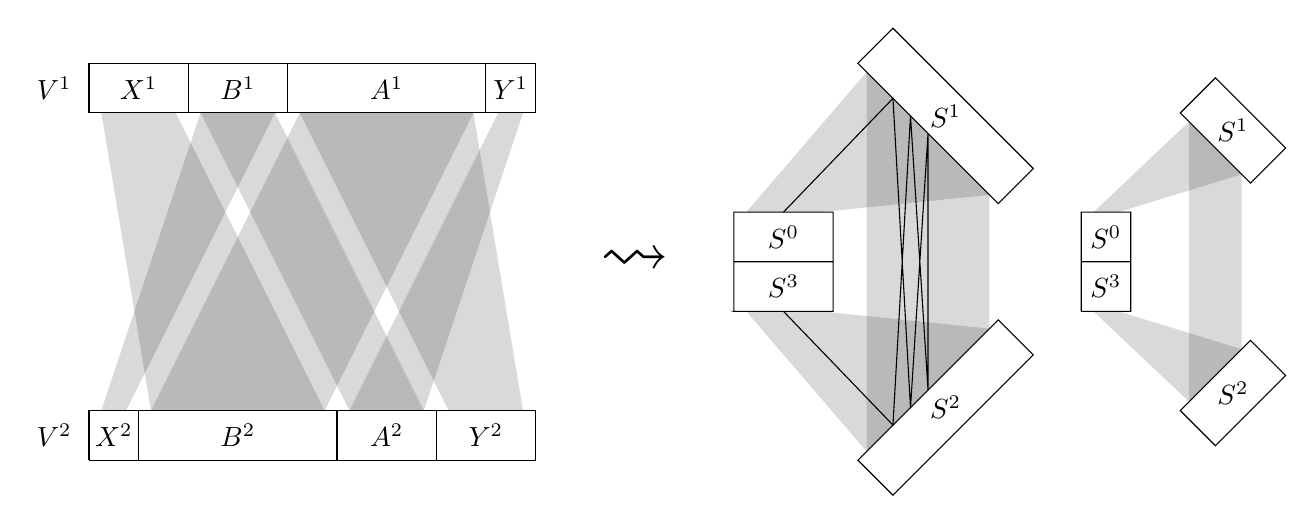
\begin{tikzpicture}[scale=0.63]

\def\y{0}
\def\h{1}
\draw (0,\y) -| (9,1+\y) -| (8,\y)
      (8,1+\y) -| (4,\y)
      (4,1+\y) -| (2,\y)
      (2,1+\y) -| (0,\y);

\node at (-0.7,0.5+\y) {$V^\h$};
\node at (1,0.5+\y) {$X^\h$};
\node at (3,0.5+\y) {$B^\h$};
\node at (6,0.5+\y) {$A^\h$};
\node at (8.5,0.5+\y) {$Y^\h$};

\def\y{-7}
\def\h{2}
\draw (0,\y) -| (9,1+\y) -| (7,\y)
      (7,1+\y) -| (5,\y)
      (5,1+\y) -| (1,\y)
      (1,1+\y) -| (0,\y);

\node at (-0.7,0.5+\y) {$V^\h$};
\node at (0.5,0.5+\y) {$X^\h$};
\node at (3,0.5+\y) {$B^\h$};
\node at (6,0.5+\y) {$A^\h$};
\node at (8,0.5+\y) {$Y^\h$};

\fill [opacity=0.15] (0.25,0) -- (1.75,0) -- (4.75,1+\y) -- (1.25,1+\y) -- cycle;
\fill [opacity=0.15] (2.25,0) -- (3.75,0) -- (0.75,1+\y) -- (0.25,1+\y) -- cycle;
\fill [opacity=0.15] (4.25,0) -- (7.75,0) -- (4.75,1+\y) -- (1.25,1+\y) -- cycle;
\fill [opacity=0.15] (2.25,0) -- (3.75,0) -- (6.75,1+\y) -- (5.25,1+\y) -- cycle;
\fill [opacity=0.15] (4.25,0) -- (7.75,0) -- (8.75,1+\y) -- (7.25,1+\y) -- cycle;
\fill [opacity=0.15] (8.25,0) -- (8.75,0) -- (6.75,1+\y) -- (5.25,1+\y) -- cycle;

\def\sqrt{1.41421356237}

\def\x{13}

\def\y{-3}
\draw (\x,\y-1) -| (\x+2,\y+1) -| cycle
      (\x,\y) -- (\x+2,\y);
\draw (\x+2.5,\y+4) -- (\x+2.5+1/\sqrt,\y+4+1/\sqrt) -- (\x+2.5+5/\sqrt,\y+4-3/\sqrt) -- (\x+2.5+4/\sqrt,\y+4-4/\sqrt) -- cycle;

\draw (\x+2.5,\y-4) -- (\x+2.5+1/\sqrt,\y-4-1/\sqrt) -- (\x+2.5+5/\sqrt,\y-4+3/\sqrt) -- (\x+2.5+4/\sqrt,\y-4+4/\sqrt) -- cycle;

\fill [opacity=0.15] (\x+0.25,\y-1) -- (\x+1.75,\y-1) -- (\x+2.5+3.75/\sqrt,\y-4+3.75/\sqrt) -- (\x+2.5+0.25/\sqrt,\y-4+0.25/\sqrt) -- cycle;
\fill [opacity=0.15] (\x+0.25,\y+1) -- (\x+1.75,\y+1) -- (\x+2.5+3.75/\sqrt,\y+4-3.75/\sqrt) -- (\x+2.5+0.25/\sqrt,\y+4-0.25/\sqrt) -- cycle;

\fill [opacity=0.15] (\x+2.5+3.75/\sqrt,\y-4+3.75/\sqrt) -- (\x+2.5+0.25/\sqrt,\y-4+0.25/\sqrt) -- (\x+2.5+0.25/\sqrt,\y+4-0.25/\sqrt) -- (\x+2.5+3.75/\sqrt,\y+4-3.75/\sqrt) -- cycle;

\draw (\x+1,\y-1) -- (\x+2.5+1/\sqrt,\y-4+1/\sqrt) -- (\x+2.5+1.5/\sqrt,\y+4-1.5/\sqrt) -- (\x+2.5+2/\sqrt,\y-4+2/\sqrt) -- (\x+2.5+2/\sqrt,\y+4-2/\sqrt) -- (\x+2.5+1.5/\sqrt,\y-4+1.5/\sqrt) -- (\x+2.5+1/\sqrt,\y+4-1/\sqrt) -- (\x+1,\y+1);

\node at (\x+1,\y+0.5) {$S^0$};
\node at (\x+1,\y-0.5) {$S^3$};
\node at (\x+2.5+2.5/\sqrt,\y+4-1.5/\sqrt) {$S^1$};
\node at (\x+2.5+2.5/\sqrt,\y-4+1.5/\sqrt) {$S^2$};

\def\x{19}
\def\y{-3}
\def\sqrt{1.41421356237}
\draw (\x+1,\y-1) -| (\x+2,\y+1) -| cycle
      (\x+1,\y) -- (\x+2,\y);
\draw (\x+3,\y+3) -- (\x+3+1/\sqrt,\y+3+1/\sqrt) -- (\x+3+3/\sqrt,\y+3-1/\sqrt) -- (\x+3+2/\sqrt,\y+3-2/\sqrt) -- cycle;

\draw (\x+3,\y-3) -- (\x+3+1/\sqrt,\y-3-1/\sqrt) -- (\x+3+3/\sqrt,\y-3+1/\sqrt) -- (\x+3+2/\sqrt,\y-3+2/\sqrt) -- cycle;

\fill [opacity=0.15] (\x+1.25,\y-1) -- (\x+1.75,\y-1) -- (\x+3+1.75/\sqrt,\y-3+1.75/\sqrt) -- (\x+3+0.25/\sqrt,\y-3+0.25/\sqrt) -- cycle;
\fill [opacity=0.15] (\x+1.25,\y+1) -- (\x+1.75,\y+1) -- (\x+3+1.75/\sqrt,\y+3-1.75/\sqrt) -- (\x+3+0.25/\sqrt,\y+3-0.25/\sqrt) -- cycle;

\fill [opacity=0.15] (\x+3+1.75/\sqrt,\y-3+1.75/\sqrt) -- (\x+3+0.25/\sqrt,\y-3+0.25/\sqrt) -- (\x+3+0.25/\sqrt,\y+3-0.25/\sqrt) -- (\x+3+1.75/\sqrt,\y+3-1.75/\sqrt) -- cycle;

\node at (\x+1.5,\y+0.5) {$S^0$};
\node at (\x+1.5,\y-0.5) {$S^3$};
\node at (\x+3+1.5/\sqrt,\y+3-0.5/\sqrt) {$S^1$};
\node at (\x+3+1.5/\sqrt,\y-3+0.5/\sqrt) {$S^2$};

\node [font=\Huge] at (11,-3) {$\rightsquigarrow$};

\end{tikzpicture}
\end{center}

\protect\caption{\label{fig:cluster-paths}From super-regular pairs to cluster-cycles.
An example special path is shown, for $k=7$.}
\end{figure}


\bibliographystyle{amsplain_initials}
\bibliography{references}

\end{document}
